\documentclass[9pt,twocolumn,twoside]{../../styles/osajnl}
\usepackage{fancyvrb}
\journal{i524} 

\title{Apache Spark's Machine Learning Library (MLlib)}

\author[1]{Anvesh Nayan Lingampalli}


\affil[1]{School of Informatics and Computing, Bloomington, IN 47408, U.S.A.}


\affil[*]{Corresponding authors: anveling@umail.iu.edu}

\dates{\today}

\ociscodes{MLlib, Apache Spark, machine learning}

% replace this with your url in github/gitlab
\doi{\url{https://github.com/Anveling/sp17-i524/paper1/S17-IR-2016/report.pdf}}


\begin{abstract}

MLlib is a machine learning library that runs on top of Apache
Spark. With Spark and MLlib, jobs that reference a number of
predefined machine learning algorithms are used to build applications.

\end{abstract}

\begin{document}

\maketitle

\section{Introduction}

Apache Spark\cite{www-spark} is a open source processing engine with
consists of elegant APIs, for performing efficient data analytics. It
provides a framework to process big data which are diverse in
nature. MLlib(Machine Learning Library) is Apache Spark's scalable
machine learning library\cite{www-mllib}. Spark has many advantages
when compared to other technologies such as Hadoop and
Storm. Hadoop\cite{www-hadoop} is a big data processing technology,
which is proved to be a solution for processing large data sets. In
cases involving machine learning or streaming data, Hadoop is not
efficient. It requires other tools such as Mahout\cite{www-mahout} or
Storm\cite{www-storm} to process the data. This is the most important
advantage that the Apache Spark has on Hadoop. Spark is faster in run
times than Hadoop MapReduce\cite{www-mapreduce}.

\begin{figure}[htbp]
\begin{center}
\centering
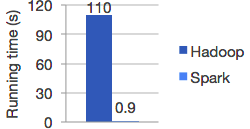
\includegraphics[width= 2.5in]{images/hadoopvspark}
\caption{Hadoop vs Spark}
\label{fig:false-color}
\end{center}
\end{figure}

Apache Spark in addition to Map and Reduce functions, also supports
SQL queries and machine learning. It has many libraries in Big Data
analytics and Machine Learning domains. MLlib is one of the top level
libraries that Spark offers.  MLlib (Machine Learning Library) is
Apache Spark’s scalable machine learning library with APIs in Java,
Python, R and Scala. It has the algorithms and tools for performing
various tasks on the data such as, clustering, classification,
regression and dimensionality reduction. The main goal of this library
is to make machine learning easy.

\section{History and Development}

Development of MLlib began in 2012 as a part of MLBase
project\cite{paper-MLBase} (Kraska et al.,
2013)\cite{www-mlbase-paper}. It is an open source since September
2013. It has since then, been integrated into the Spark as an in-built
package. The original version of MLlib was developed in UC Berkeley
and provided a limited set of machine learning methods. Since it is an
open source community, MLlib developed and now has additional
functionality.
 

\section{Components of MLlib}

MLib provides various linear models, Naive bayes\cite{www-naivebayes}
and decision trees\cite{www-decisiontrees} for classification and
regression problems. With the help of these models, problems such as
alternating least squares(ALS), k-means
problem\cite{www-kmeansproblem}, PCA (principal component
analysis)\cite{www-pca} for clustering have been successfully
implemented. Text mining, predictive analysis of data are certain
areas where MLlib is being used as an efficient tool.

MLlib has a package named spark.ml, which provides APIs for the
functionality of the pipelines. This package enables users to swap the
existing algorithms with their own algorithms\cite{MLlib-article}.

MLlib supports various methods for binary classification, multiclass
classification, and regression analysis. Each type of problem has its
own supported algorithms. Binary Classification has Linear SVMs,
Logistic regression\cite{www-logisticregression}, decision trees and
naive Bayes. Multiclass Classification also has decision trees and
naive Bayes as its supported algorithms. Regression has linear least
squares\cite{www-linearleastsquares}, Lasso\cite{www-lasso} and
decision trees.

\section{Performance analysis between MLlib and its alternatives}
Hadoop Mahout is one of the alternative choice for a machine learning
library. Mahout uses Hadoop as underlying framework whereas in the
case of MLlib, it is Spark. In terms of features, support and
performance MLlib performs better. In 2014, Mahout announced it would
not accept Hadoop MapReduce and completely switched to Spark.

H2O\cite{www-H2O}, xgboost\cite{www-xgboost}, python
scikit-learn\cite{www-scikitlearn} are few other alternatives to
MLlib. Scalability, speed and performance are measured for these tools
and are shown in the table.

\begin{figure}[htbp]
\begin{center}
\centering
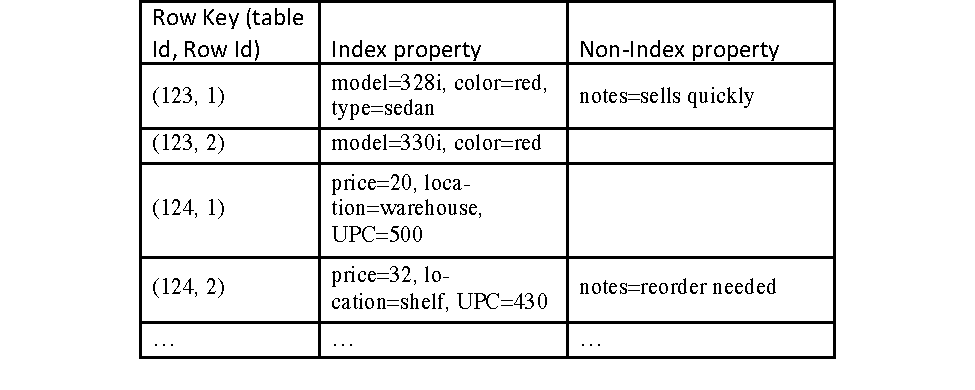
\includegraphics[width= \linewidth, height = 2.5in]{images/table1}
\caption{Analysis of performance}
\label{fig:false-color}
\end{center}
\end{figure}

For each tool and each size N, observations of the training tie,
memory usage, and accuracy are presented. These tests have been
carried out on a Amazon EC2 instance (32 cores, 60GB
RAM)\cite{Analysis-webpage}.

The graph for the results is shown below. H2O is memory efficient and
faster than MLlib. But, MLlib is the better choice of the two as it has
variety of functionalities.

\begin{figure}[htbp]
\begin{center}
\centering
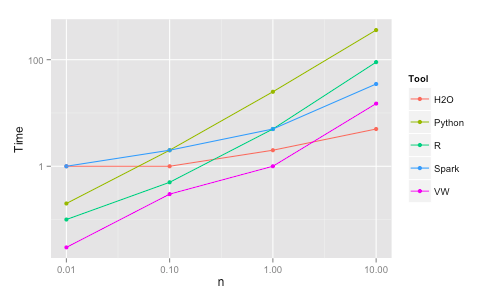
\includegraphics[width=\linewidth]{images/analysisgraph}
\caption{Graph analysis}
\label{fig:false-color}
\end{center}
\end{figure}

\section{Use Cases}
Apache Spark Machine Learning Library is used in wide range of
applications in research and industry. Here two such applications are
described briefly.

\subsection{Movie Recommendation with MLlib}
In this mini course project MLlib library is used to make personalized
movie recommendations.\cite{MovieRecommender}

\subsection{Predict Telco Churn with Apache Spark MLlib}

Churn prediction\cite{www-churnprediction}, is one of the most common
applications of machine learning in the telecommunications industry,
as well as many other subscriptions-based industries.MLlib is used
here to fit a machine-learning model that can predict which customers
of a telecommunications company are likely to stop using their
service.\cite{TelcoChurn}

\section{Useful Resources}

\cite{www-mllib-guide} also
has some good step by step tutorials on how to use Machine learning
library to work on big data anlytics involving machine learning
learning studio.

\section{Conclusion}

In conclusion, MLlib is a library used to perform machine learning as
a part of big data analysis. It is designed for simplicity,
scalability, and easy integration with other tools It is still in
active development phase, and there have been many improvements over
the previous versions over time. MLlib provides developers with a wide
range of tools to make machine learning easy and scalable.

\section{Acknowledgements}

This work was done as part of the course "I524: Big Data and Open
Source Software Projects" at Indiana University during Spring
2017. 

\bibliography{references}

\end{document}
